\chapter{Opis metody źródeł pozornych}\label{cha:ims}

%---------------------------------------------------------------------------

\section{Wprowadzenie}\label{sec:wprowadzenie}

Metoda źródeł pozornych jest jedną z metod często wykorzystywanych w~akustyce architektonicznej i~cyfrowym przetwarzaniu sygnałów. Przy użyciu tej metody możemy wygenerować odpowiedź impulsową pomieszczenia, zbadać dyfuzyjność pola  czy prześledzić ścieżkę propagacji dźwięku. Ze względu na liczne uproszczenia, w~metodzie nie jest uwzględnianych wiele zjawisk falowych. W jej najprostszej implementacji pomijane są takie zjawiska jak dyfrakcja, interferencja czy rozproszenie fali. W wielu przypadkach, aby ta metoda była skuteczna, należy przeprowadzić złożone obliczenia lub wykorzystać ją równolegle z innymi metodami numerycznymi.


%---------------------------------------------------------------------------

\section{Główne założenia metody}\label{sec:gzm}

W przypadku metod geometrycznych falę dźwiękową modelujemy jako prosty obiekt przestrzenny. W metodzie źródeł pozornych punktowe źródło zastępujemy nieskończonym zbiorem półprostych. Każdy taki promień dźwiękowy reprezentuje pewną część składową fali i~jej kierunek propagacji. Każda składowa odbija się od powierzchni zgodnie z prawem Snella, a~przy odbiciu zostaje pochłonięta część jej energii proporcjonalna do współczynnika pochłaniania dźwięku dla danego materiału. Kolejnym założeniem jest, że powierzchnie odbijające są powierzchniami płaskimi, a~w~polu występuje jedno  punktowe źródło i~jeden punkt odbioru. W przypadku większej ilości punktów obserwacji lub większej ilości źródeł należałoby skorzystać z szerszych metod, jakimi są metoda obrazów pozornych i~metoda pozornych obrazów punktu obserwacji. Przy powyższych założeniach  każdą ścieżkę propagacji promienia dźwiękowego można zastąpić pozornym źródłem. Źródło pozorne dla danej składowej fali powstaje w~wyniku odbicia lustrzanego punktu źródła względem powierzchni odbijającej tą składową. W przypadku większej ilości odbić punkt źródła należy odbić lustrzanie względem każdej kolejnej powierzchni odbijającej. Zbiór wyznaczonych w~ten sposób źródeł nazywamy siatką źródeł pozornych, która reprezentuje warunki akustyczne analizowanego pomieszczenia dla ściśle określonych punktów źródła i~odbioru. Siatka źródeł pozornych może być podstawą do wyznaczenia echogramu i~czasu pogłosu pomieszczenia. Ze względu na dużą złożoność obliczeniową metody często uzyskiwane są wyniki, które nie wystarczają do analizy pola akustycznego. W tym wypadku stosuje się połączenie kilku metod numerycznych~\cite{b11}~\cite{b12}~\cite{b13}~\cite{b14}.

%---------------------------------------------------------------------------

\section{Wyznaczanie siatki źródeł pozornych}\label{sec:szp}

W celu wyznaczenia siatki źródeł pozornych N-tego rzędu zdefiniujmy punkt źródła dźwięku $S$, punkt odbioru $R$ oraz K-liczny zbiór powierzchni odbijających $P_i$ gdzie $i$ oznacza numer powierzchni (Rys. 2.1.). 

\begin{figure}[H]
        \centering
                \centering
                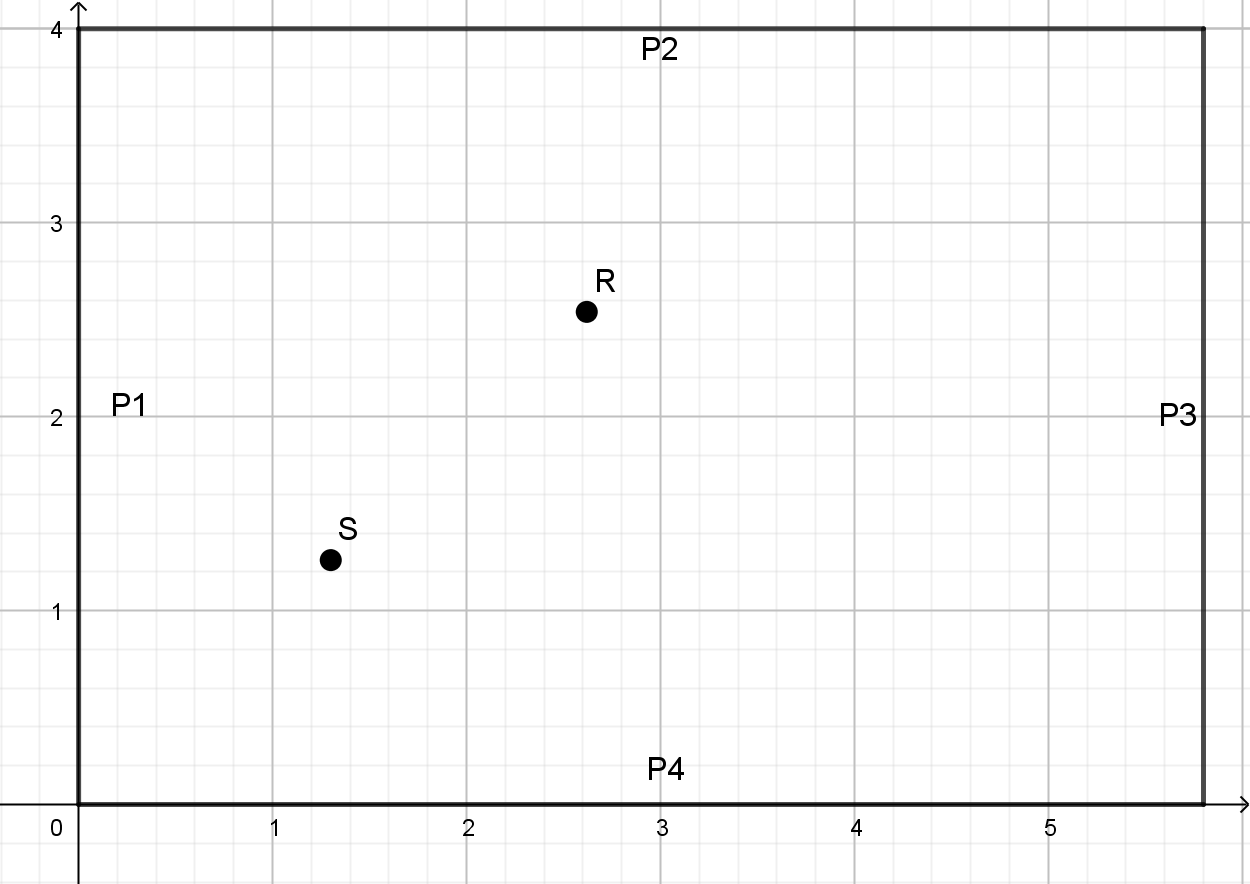
\includegraphics[width=12cm]{rys1}
	\caption{Model geometrii pomieszczenia (S - punkt źródła dźwięku, R - punkt obserwacji, Pn - kolejne powierzchnie odbijające).}
\end{figure}

Do znalezienia wszystkich źródeł pozornych N-tego rzędu należy wygenerować wszystkie $K^N$ wariacje z powtórzeniami zbioru $P$. Na wstępie możemy pominąć wariacje, w~których ta sama powierzchnia jest przynajmniej dwoma kolejnymi elementami ciągu, ponieważ promień dźwiękowy nie może dwukrotnie z rzędu odbić się od tej samej powierzchni. Każda wariacja reprezentuje jeden promień dźwiękowy, który odbija się kolejno od każdej powierzchni w~wariacji. Aby znaleźć źródło pozorne dla danego promienia dźwiękowego należy odbić punkt źródła symetrycznie względem każdej z płaszczyzn w~wariacji (Rys. 2.2.). 

\begin{figure}[H]
        \centering
                \centering
                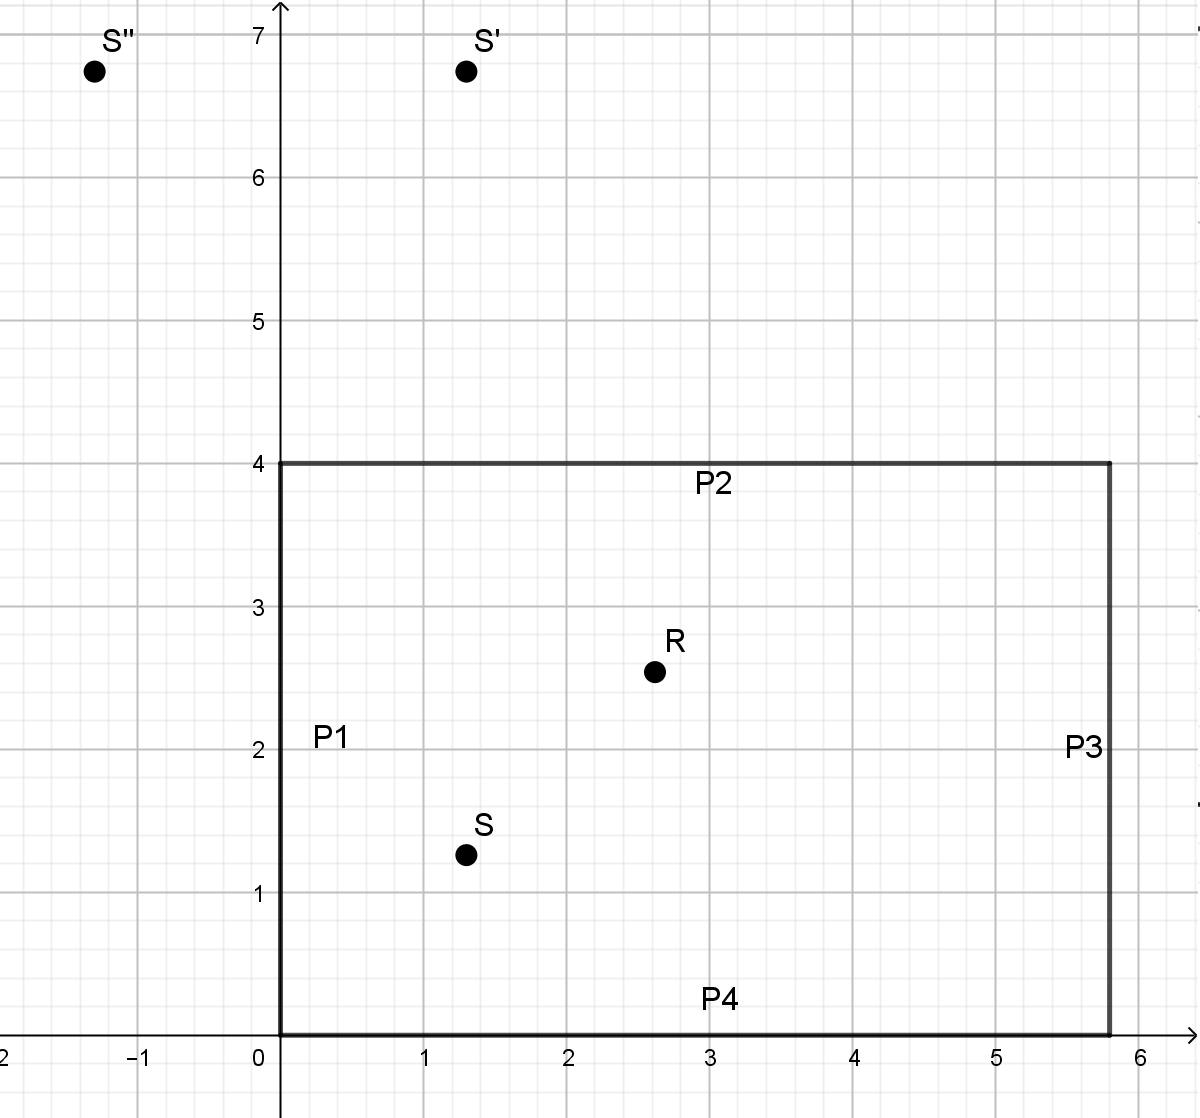
\includegraphics[width=12cm]{rys2}
	\caption{Pierwsze i~drugie odbicie względem powierzchni  (S - punkt źródła dźwięku, S' i S'' - kolejne odbicia symetryczne punktu S względem powierzchni odbijających, R - punkt obserwacji, Pn - kolejne powierzchnie odbijające).}
\end{figure}

Dla uzyskanego punktu należy zweryfikować, czy promień dźwiękowy jest w~stanie dotrzeć od punktu źródła do punktu odbiornika w~danym układzie geometrycznym. W tym celu należy prześledzić ścieżkę promienia dźwiękowego wstecz – zaczynając od punktu obserwacji. Początkowy kierunek promienia znajduje się wyznaczając wektor rozpięty od punktu źródła pozornego do punktu obserwacji. Prosta przechodząca przez te punkty powinna przecinać ostatnią powierzchnię z wariacji. Kąt pomiędzy wektorem wyznaczającym kierunek ścieżki promienia dźwiękowego a~wektorem normalnym płaszczyzny, na której leży powierzchnia odbijająca, powinien być mniejszy niż 90 stopni. Odcinek łączący punkt obserwacji z punktem przecięcia powyższej prostej z powierzchnią odbijającą stanowi fragment ścieżki promienia dźwiękowego. Kolejny fragment ścieżki promienia dźwiękowego wyznacza się odbijając symetrycznie poprzedni odcinek względem kolejnej powierzchni odbijającej. Z każdym krokiem należy sprawdzić czy odcinek ścieżki promienia dźwiękowego przecina płaszczyzny względem których się odbija. Jeśli uda się prześledzić ścieżkę promienia dźwiękowego od punktu obserwacji do punktu źródła, można sprawdzany punkt uznać za źródło pozorne i~uwzględnić w~siatce źródeł pozornych.

%---------------------------------------------------------------------------

\section{Uwzględnienie współczynnika pochłaniania}\label{sec:zm}

W akustyce architektonicznej, przy symulacji warunków akustycznych w~pomieszczeniu, istotne jest uwzględnienie współczynnika pochłaniania dźwięku (Wzór 2.1.). \\

\begin{equation}
\alpha=\frac{E_{poch}}{E_{pad}}
\end{equation}
gdzie
\begin{eqwhere}[2cm]
        \item[$E_{poch}$] energia fali pochłoniętej
        \item[$E_{pad}$] energia fali padającej
\end{eqwhere}

Definiując dla każdej powierzchni odbijającej współczynnik pochłaniania $\alpha_i$, gdzie $i$  jest indeksem powierzchni, możemy dla każdej z nich wyznaczyć współczynnik odbicia $R_i$. Mnożąc przez siebie współczynniki odbić fali dla kolejnych powierzchni i~przemnażając przez energię źródła otrzymujemy energię źródła pozornego odpowiadającego odbiciom od powyższych powierzchni (Wzór 2.2). \\

\begin{equation}
E_{IS}=E_{S}\cdot\prod_{i=1}^{N}(1-\alpha_i)
\end{equation}
gdzie
\begin{eqwhere}[2cm]
        \item[$E_{S}$] energia źródła dźwięku
        \item[$N$] liczba powierzchni odbijających
        \item[$\alpha_i$] współczynniki pochłaniania kolejnych powierzchni odbijających
\end{eqwhere}

%---------------------------------------------------------------------------

\section{Przykładowe użycie metody}\label{sec:przyuzy}

Przyjmując prostopadłościenne pomieszczenie z umieszczonym punktowym źródłem dźwięku i~punktem obserwacji (Rys. 2.3.), wyznaczamy siatkę źródeł pozornych (Rys. 3.4.). Dla przejrzystości rysunku siatka została wyznaczona dla maksymalnie trzeciego odbicia.
 
\begin{figure}[H]
        \centering
                \centering
                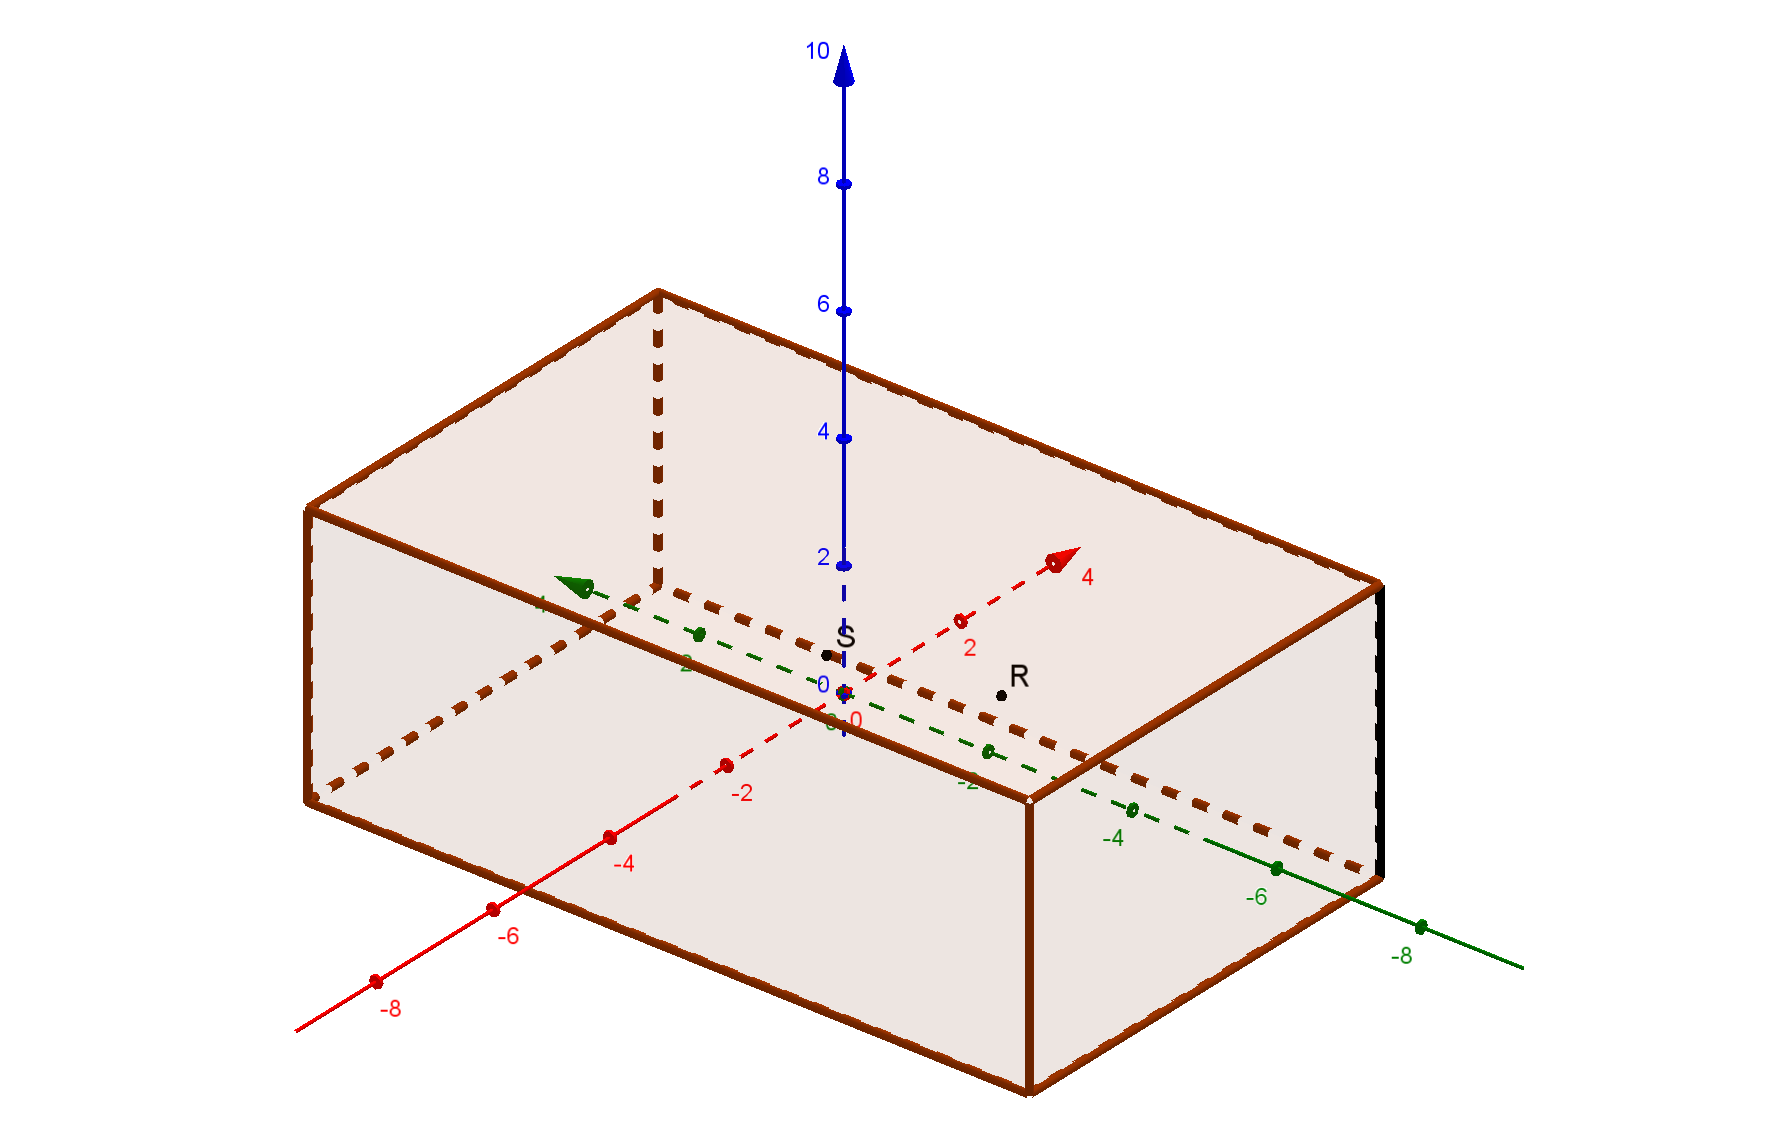
\includegraphics[width=12cm]{rys3}
	\caption{Model geometrii pomieszczenia (S - punkt źródła dźwięku, R - punkt obserwacji).}
\end{figure}

\begin{figure}[H]
        \centering
                \centering
                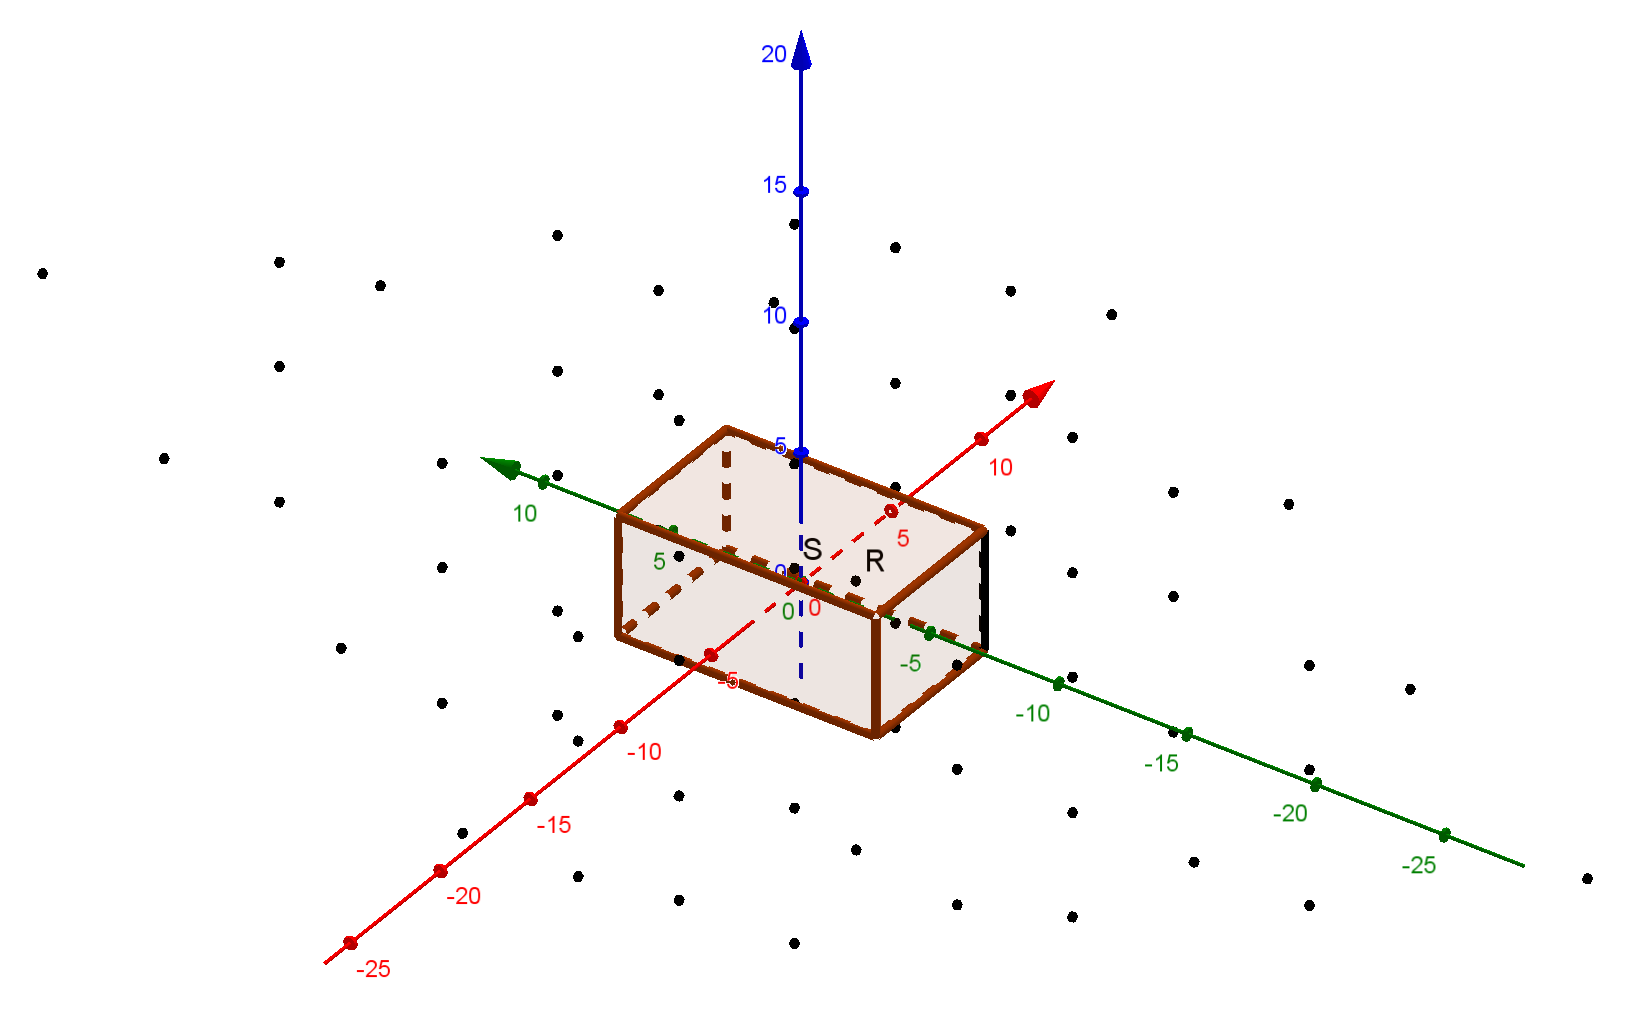
\includegraphics[width=12cm]{rys4}
	\caption{Siatka źródeł pozornych (S - punkt źródła dźwięku, R - punkt obserwacji).}
\end{figure}

Położenia  źródeł pozornych w~siatce dają informację o kierunkach promieni dźwiękowych dochodzących do punktu obserwacji. Uwzględniając straty energii pochłoniętej przez odbicia oraz starty energii związanej z rozchodzeniem się fali kulistej możemy wyznaczyć  ilość energii i~czas, w~jakim dotrze ona do punktu obserwacji dla każdego źródła pozornego. Zależność energii dochodzącej do punktu odbioru od czasu przedstawiona jest na poniższym echogramie (Rys. 2.5.).

\begin{figure}[H]
        \centering
                \centering
                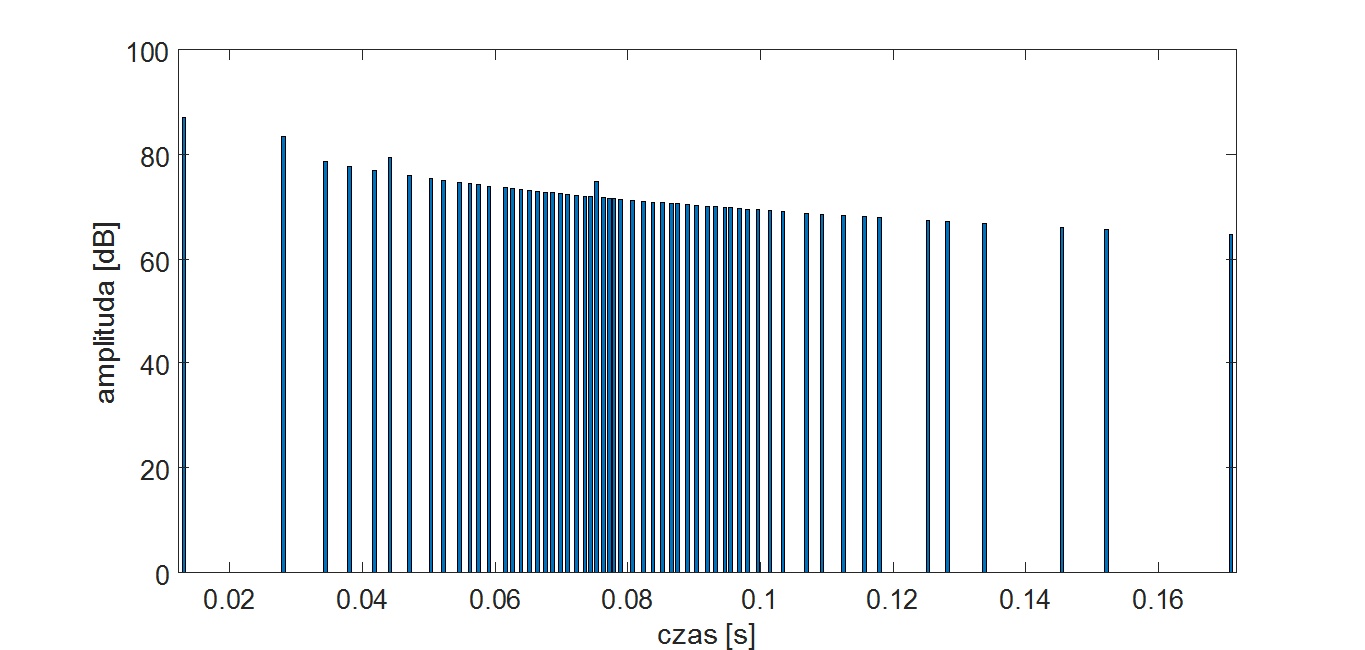
\includegraphics[width=16cm]{rys5}
	\caption{Echogram.}
\end{figure}

Uzyskany echogram lub jego część mogą być użyte do obliczenia wskaźników C50, C80, D50. Poprzez całkowanie wsteczne echogramu można uzyskać krzywą zaniku energii dźwięku w~pomieszczeniu (Rys. 2.6.).

\begin{figure}[H]
        \centering
                \centering
                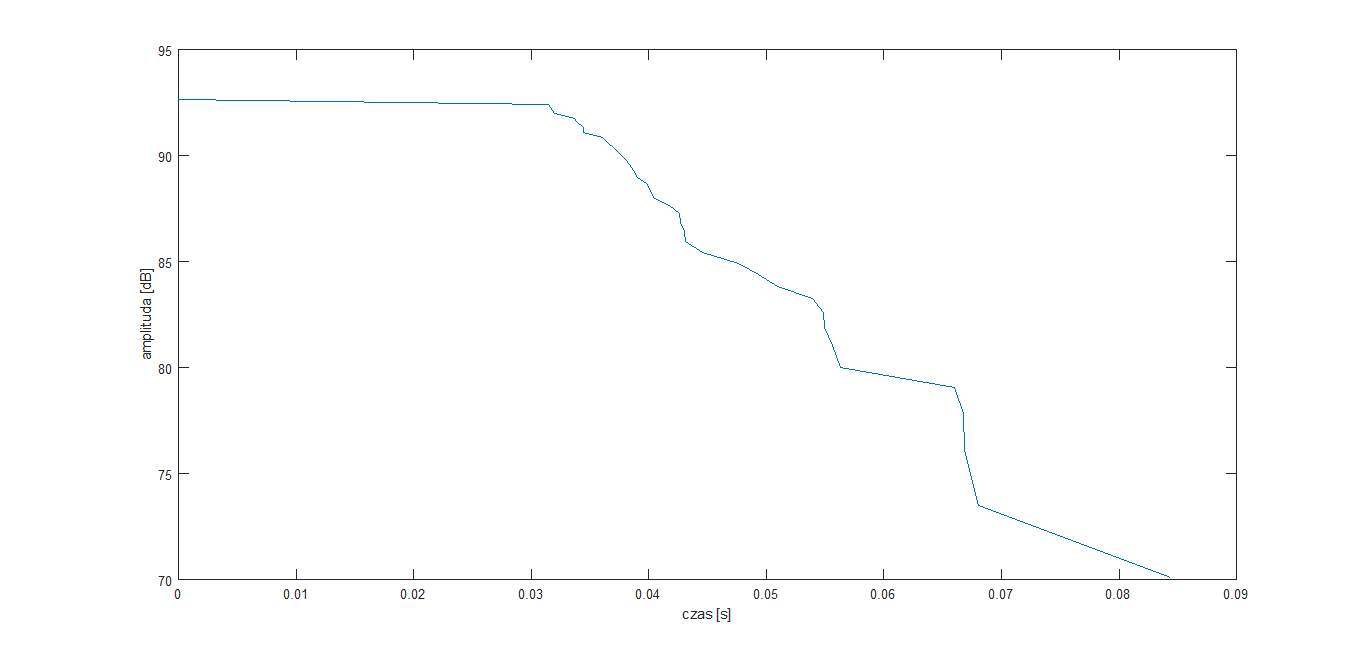
\includegraphics[width=16cm]{rys6}
	\caption{Krzywa zaniku dźwięku.}
\end{figure}

Na jej podstawie można wyznaczyć czas pogłosu pomieszczenia. W porównaniu do metody źródeł pozornych, w~metodzie promieniowej, ze względu na mniejszą złożoność obliczeń, uzyskuje się dłuższe echogramy. Zaletą metody źródeł pozornych jest uzyskiwanie dokładnych ścieżek promieni dźwiękowych, a~nie, jak w~przypadku metody promieniowej, ścieżek trafiających jedynie w~okolice punktu obserwacji. Ze względu na zalety obu tych metod często stosuje się je łącznie~\cite{b13}~\cite{b14}.















